%----------------------------------------------------------------------------------------
% PACKAGES AND DOCUMENT CONFIGURATIONS
%----------------------------------------------------------------------------------------

  \documentclass{article}

  \usepackage{hyperref}
  \usepackage{fancyhdr} % Required for custom headers
  \usepackage{lastpage} % Required to determine the last page for the footer
  \usepackage{extramarks} % Required for headers and footers
  \usepackage[usenames,dvipsnames]{color} % Required for custom colors
  \usepackage{graphicx} % Required to insert images
  \usepackage{listings} % Required for insertion of code
  \usepackage{courier} % Required for the courier font
  \usepackage{lipsum} % Used for inserting dummy 'Lorem ipsum' text into the template
  \usepackage{wrapfig}
  \usepackage{color}
  \usepackage{lscape}

  \setlength\parindent{0pt} % Removes all indentation from paragraphs
  \renewcommand{\labelenumi}{\alph{enumi}.} % Make numbering in the itemize environment by letter rather than number (e.g. section 6)

  % Margins
  \topmargin=-0.7in
  \evensidemargin=0.2in
  \oddsidemargin=-0.2in
  \textwidth=7.0in
  \textheight=9.3in
  % \headsep=0.25in

  % \linespread{1.1} % Line spacing

  \definecolor{dkgreen}{rgb}{0,0.6,0}
  \definecolor{gray}{rgb}{0.5,0.5,0.5}
  \definecolor{mauve}{rgb}{0.58,0,0.82}
  \definecolor{greyish}{rgb}{0.96,0.96,0.96}

  \lstset{
    backgroundcolor=\color{greyish},   % choose the background color; you must add \usepackage{color} or \usepackage{xcolor}
    frame=tb,
    numbers=left,                    % where to put the line-numbers; possible values are (none, left, right)
    numbersep=5pt,                   % how far the line-numbers are from the code
    numberstyle=\tiny\color{mygray}, % the style that is used for the line-numbers
    language=Ruby,
    aboveskip=3mm,
    belowskip=3mm,
    showstringspaces=false,
    columns=flexible,
    basicstyle={\footnotesize\ttfamily},
    numbers=none,
    numberstyle=\tiny\color{gray},
    keywordstyle=\color{blue},
    commentstyle=\color{dkgreen},
    stringstyle=\color{mauve},
    breaklines=true,
    breakatwhitespace=true
    tabsize=3
  }
  \lstset{basicstyle=\ttfamily\footnotesize,breaklines=true}
%----------------------------------------------------------------------------------------
% DOCUMENT INFORMATION
%----------------------------------------------------------------------------------------
  \begin{document}
  \begin{titlepage}

%----------------------------------------------------------------------------------------
% TITLE PAGE INFORMATION
%----------------------------------------------------------------------------------------
 \newcommand{\HRule}{\rule{\linewidth}{0.5mm}} % Defines a new command for the horizontal lines, change thickness here
  \begin{center} % Center everything on the page

  %----------------------------------------------------------------------------------------
  % HEADING SECTIONS
  %----------------------------------------------------------------------------------------
  \textsc{\Large Faculty of Computers, Informatics and Microelectronics}\\[0.5cm]
  \textsc{\LARGE Technical University of Moldova}\\[1.2cm] % Name of your university/college
  \vspace{25 mm}
  \textsc{\Large SI}\\[0.5cm] % Major heading such as course name
  %\textsc{\large Laboratory work \#1-3}\\[0.5cm] % Minor heading such as course title
  \textsc{\large Laboratory work \# 3}\\[0.5cm] % Minor heading such as course title

  %----------------------------------------------------------------------------------------
  % TITLE SECTION
  %----------------------------------------------------------------------------------------
  \vspace{10 mm}
  \HRule \\[0.4cm]
  { \LARGE \bfseries Diffie–Hellman key exchange }\\[0.4cm] % Title of your document
  \HRule \\[1.5cm]

  %----------------------------------------------------------------------------------------
  % AUTHOR SECTION
  %----------------------------------------------------------------------------------------
  \vspace{40mm}

  \begin{minipage}{0.4\textwidth}
  \begin{flushleft} \large
  \emph{Author:}\\
  Petru \textsc{Negrei} % Your name
  \end{flushleft}
  \end{minipage}
  ~
  \begin{minipage}{0.4\textwidth}
  \begin{flushright} \large
  \emph{Supervisor:} \\
  A. \textsc{Railean} % Supervisor's Name
  \end{flushright}
  \end{minipage}\\[4cm]

  \vspace{15 mm}
  % If you don't want a supervisor, uncomment the two lines below and remove the section above
  %\Large \emph{Author:}\\
  %John \textsc{Smith}\\[3cm] % Your name

  %----------------------------------------------------------------------------------------
  % DATE SECTION
  %----------------------------------------------------------------------------------------

  {\large November 2014}\\[3cm] % Date, change the \today to a set date if you want to be precise

  %----------------------------------------------------------------------------------------
  % LOGO SECTION
  %----------------------------------------------------------------------------------------

  %\includegraphics{Logo}\\[1cm] % Include a department/university logo - this will require the graphicx package

  %----------------------------------------------------------------------------------------

  \vfill % Fill the rest of the page with whitespace
  \end{center}
  \end{titlepage}

  % \newpage
  % \tableofcontents
  % \newpage

%----------------------------------------------------------------------------------------
% Introduction
%----------------------------------------------------------------------------------------

  \section{Introduction}

  \subsection{Objective}

  Construct the Diffie–Hellman key exchange algorithm.

  \subsection{Definition}

  \textbf{Diffie–Hellman key exchange} (D–H)is a specific method of exchanging cryptographic keys. It is one of the earliest practical examples of key exchange implemented within the field of cryptography.
   The Diffie–Hellman key exchange method allows two parties that have no prior knowledge of each other to jointly establish a shared secret key over an insecure communications channel. 
   This key can then be used to encrypt subsequent communications using a symmetric key cipher.

%%--------------------------------------------------------------------------
%% Implementation
%%--------------------------------------------------------------------------

  \section{Description}


  \begin{minipage}[b]{0.5\linewidth}
    Diffie–Hellman establishes a shared secret that can be used for secret communications while exchanging data over a public network. 
    The following diagram illustrates the general idea of the key exchange by using colors instead of a very large number.
    The crucial part of the process is that Alice and Bob exchange their secret colors in a mix only. Finally this generates an identical key that is computationally difficult 
    to reverse for another party that might have been listening in on them. Alice and Bob now use this common secret to encrypt and decrypt their sent and received data.
    \vspace{4cm}
  \end{minipage}
  \begin{minipage}[b]{0.5\linewidth}
    \begin{center}
      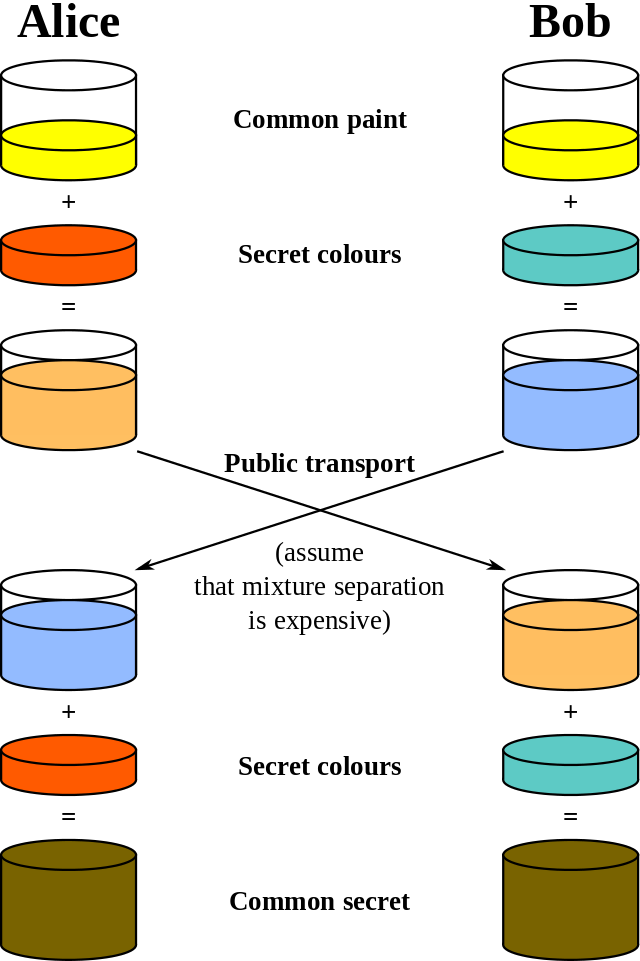
\includegraphics[width=0.6\textwidth]{dh}
      \\ Illustration of the Diffie–Hellman Key Exchange
    \end{center}
  \end{minipage}

  \section{Implementation}

  Although  there is an implementation of the Diffie-Hellman key exchange protocol in ruby OpenSSL module. I implemented the algorithm again using
  small numbers for testing.

    \begin{lstlisting}
    require 'prime'

    # an implementation of the Diffie-Hellman key exchange protocol
    module OpenSSL

        # p -  prime. g- generator 
        # pub_key - per-session public key matching the private key
        # this needs to be passed to #compute_key.
        # #priv_key - per-session private key
        attr_reader :p, :g, :priv_key

        class DH

            def initialize str="#{p}:#{g}"
                @p, @g = str.split(":").map(&:to_i)
            end

            def priv_key
                @priv_key ||= rand(1000) + 1
            end

            def to_der
                "#{p}:#{g}"
            end

            def generate_key!
                @pub_key ||= (g**priv_key) % p
            end

            def compute_key pub_key
                (pub_key ** priv_key) % p
            end

            def p
                @p ||= Prime.each(10**3).to_a.sample
            end

            def g 
                5 # or something else
            end

            def pub_key 
              @pub_key 
            end
        
        end
    end
    \end{lstlisting}

    Verification of working algorithm. 

    \begin{lstlisting}
      dh1 = OpenSSL::DH.new
      dh1.generate_key!                                      #generate the per-session key pair
      der = dh1.to_der                                       #you may send this publicly to the participating party
      dh2 = OpenSSL::DH.new(der)
      dh2.generate_key!                                      #generate the per-session key pair

      symm_key1 = dh1.compute_key(dh2.pub_key)
      symm_key2 = dh2.compute_key(dh1.pub_key)

      puts symm_key1 == symm_key2                            # => true
    \end{lstlisting}

 \section{Conclussion}


    After making this laboratory work I learn about Diffie–Hellman method of exchanging cryptographic keys. 
    The protocol is considered secure against eavesdroppers if G and g are chosen properly, the order of G should 
    have a large prime factor to prevent use of the Pohlig–Hellman algorithm. Also if parties use random number 
    generators whose outputs are not completely random there is a possibility to predict to some extent.



\end{document}

